\chapter{Il Livello Applicazione}
\thispagestyle{chapterInit}
\paragraph{Obbiettivi}
    \begin{itemize}
        \item Capire i principi che sono alla base dei servizi di livello di trasporto:
            \subitem Multiplexing/de-multiplexing
            \subitem Trasferimento dati affidabile
            \subitem Controllo di flusso
            \subitem Controllo di congestione
        \item Descrivere i protocolli del livello di trasporto di Internet:
            \subitem TCP: Trasposto orientato alla connessione
            \subitem Controllo di congestione TCP
            \subitem UDP: Trasporto non orientato alla connessione
    \end{itemize}
\section{Servizi a livello di trasporto}
    \paragraph{Introduzione} I \textbf{protocolli di trasporto} forniscono la comunicazione logica tra processi applicativi di host diversi. I protocolli di trasporto vengono eseguiti negli host "terminali" ovvero quelli che generano o consumano i dati. Dal lato di inviante il protocollo di trasporto divide in diversi segmenti i dati ricevuti dal livello di applicazione e li invia al livello di rete. Dal lato di ricevente il protocollo di trasporto riassembla i segmenti ricevuti e li invia al livello di applicazione.
    \paragraph{TCP} Il \textbf{TCP} (Transmission Control Protocol) è un protocollo di trasporto orientato alla connessione. Il TCP fornisce un trasferimento affidabile dei dati, controllo di flusso e controllo di congestione.
    \paragraph{UDP} L'\textbf{UDP} (User Datagram Protocol) è un protocollo di trasporto non orientato alla connessione. L'UDP non fornisce trasferimento affidabile dei dati, controllo di flusso e controllo di congestione.
    \paragraph{Servizi non disponibili} Al momento in internet non è disponibile un servizio di garanzia su ritardi (latenza), e non è disponibile un servizio di garanzia sulla banda (velocità di trasferimento).
\section{Multiplexing e De-multiplexing}
    \paragraph{Introduzione} Il \textbf{multiplexing} è il processo di invio di dati da più socket a un'unica connessione, per identificare il socket di destinazione si utilizza un \textbf{port number}. Il \textbf{de-multiplexing} è il processo di invio dei dati ricevuti al socket corretto in base al port number.
    \subsection{De-multiplexing}
        \paragraph{Come funziona} In primo luogo quando l'\textit{host} riceve un segmento IP contenente: IP del mittente, IP del destinatario, protocollo di trasporto, porta di destinazione e porta di sorgente. L'\textit{host} utilizza l'indirizzo IP del destinatario e la porta di destinazione per inviare il segmento al processo corretto.
        \subsubsection{De-multiplexing senza connessione}
            Per eseguire il de-multiplexing senza connessione si crea un socket per ricevere i dati. Il socket è ora associato a una porta ed a un indirizzo IP. Quando l'\textit{host} riceve il segmento \texttt{UDP}, viene controllato che il numero di porta di destinazione sia uguale alla porta del socket. Se il numero di porta non corrisponde il segmento viene scartato. Se invece il numero di porta corrisponde il segmento viene inviato al processo associato al socket.
            \begin{figure}[H]
                \centering
                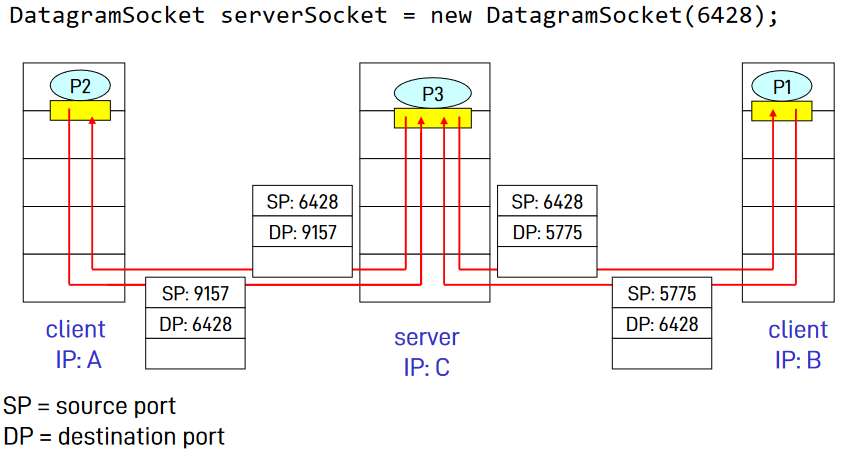
\includegraphics[width=0.5\textwidth]{03/DemultiplexingSenzaConnessione.png}
                \caption{De-multiplexing senza connessione}
            \end{figure}
        \subsubsection{De-multiplexing orientato alla connessione}
            Quando si utilizza un protocollo orientato alla connessione (\texttt{TCP}), il processo di de-multiplexing è leggermente diverso. Il socket infatti è costituito da quattro parametri: indirizzo IP del mittente, indirizzo IP del destinatario, numero di porta di sorgente e numero di porta di destinazione. Quando l'\textit{host} riceve un segmento \texttt{TCP} controlla che i quattro parametri del socket corrispondano ai quattro parametri del segmento. Se i parametri non corrispondono il segmento viene scartato, altrimenti viene inviato al processo associato al socket. Un \textit{host} può supportare più socket contemporaneamente purché cambi almeno uno dei quattro parametri, inoltre i \textit{web server} sono un chiaro esempio di applicazione che utilizza più socket contemporaneamente (su \texttt{HTTP/1.0} un socket per ogni richiesta).\footnote{Se viene allocata una porta ad una connessione, la porta non può essere utilizzata da altre connessioni, quindi nel caso di un \textit{web server} è vero che questo ascolta sulla porta 80, ma quando un client si connette al server, il server apre un socket con una porta dinamica.}
            \begin{figure}[H]
                \centering
                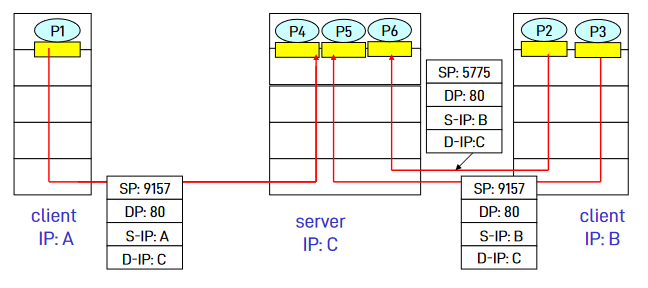
\includegraphics[width=0.5\textwidth]{03/DemultiplexingConConnessione.png}
                \caption{De-multiplexing orientato alla connessione}
            \end{figure}
    \subsection{Porte \texttt{TCP}-\texttt{UDP}}
        La destinazione finale di un segmento non è un host ma un processo. L'interfaccia tra l'applicazione e il livello di trasporto è chiamata \textbf{socket} o \textbf{porta} (nel caso di \texttt{UDP} e \texttt{TCP}). Un \textbf{socket} è un indirizzo IP e un numero di porta. Un \textbf{port number} è un numero a 16 bit che identifica un processo all'interno di un host. Esiste una mappatura biunivoca tra un \textbf{port number} e un processo. I servizi standard utilizzano porte ben note con valori tra 0 e 1023. I processi non-standard e le connessioni in ingresso a un client usano numeri fino a 25535 (16 bit).
        \paragraph{Numeri di porte}
            I numeri di porta si classificano come segue:
            \begin{description}
                \item[Statici] Per i servizi standard, es. HTTP (80), FTP (21), SSH (22), Telnet (23), SMTP (25), POP3 (110), IMAP (143), HTTPS (443), ecc.
                \item[Dinamici] (o "ephemeral") per le connessioni in uscita o per porte allocate dinamicamente, es. client web, client FTP, client SSH, client Telnet, client SMTP, client POP3, client IMAP, client HTTPS, ecc.
            \end{description}
            Inoltre è importante dire che le porte di sorgente e di destinazione non sono le stesse in quanto la porta di sorgente è una porta dinamica assegnata dal sistema operativo.
\section{Trasporto senza connessione: \texttt{UDP}}
    \paragraph{Caratteristiche} L'\textbf{UDP} (User Datagram Protocol) è un protocollo di trasporto senza connessione, offre un servizio \textit{best effort} e non fornisce garanzie di consegna, ordine o duplicazione dei dati. Questo in quanto non ha \textit{handshake} iniziale e non mantiene alcuno stato di connessione. 
    \paragraph{Perché esiste \texttt{UDP}} Non richiede di stabilire una connessione, è semplice e veloce, Header di segmento corti, senza controllo di congestione.
    \subsection{Header}
        \begin{figure}[H]
            \centering
            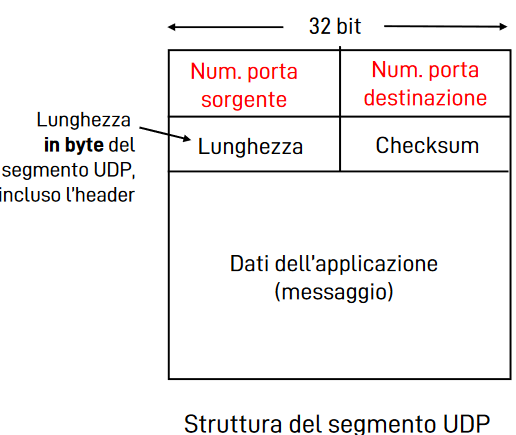
\includegraphics[width=0.3\textwidth]{03/UDPHeader.png}
            \caption{Header di un segmento UDP}
        \end{figure}
        \begin{description}
            \item[Porta di sorgente] Numero di porta del processo mittente.
            \item[Porta di destinazione] Numero di porta del processo destinatario.
            \item[Lunghezza] Lunghezza del segmento in byte.
            \item[Checksum] Utilizzato per rilevare errori nel segmento.
        \end{description}
        \subsubsection{Checksum}
            Il checksum è un campo a 16 bit che viene utilizzato per rilevare errori nel segmento. Questo viene calcolato da entrambe le parti: viene trattato il contenuto come una sequenza di $ 16 $ bit e si sommano tutti i bit (se presente riporto questo viene sommato a sua volta) e viene eseguito il complemento a 1. Il mittente invia il checksum calcolato nel segmento e il ricevente calcola il checksum del segmento ricevuto e lo confronta con il checksum ricevuto. Se i due checksum non corrispondono il segmento viene scartato.
\section[trasferimento dati affidabile]{Principi del trasferimento dati affidabile}
    \subsection{\texttt{ARQ}}
        \textbf{\texttt{ARQ}} o \textit{Automatic Repeat reQuest} è una classe di protocolli che "cercano" di recuperare i segmenti persi o danneggiati. Questa classe usa dei pacchetti speciali per notificare al mittente che un segmento è stato perso o danneggiato. Questi pacchetti speciali sono chiamati \texttt{ACK} (Acknowledgement) e \texttt{NACK} (Negative Acknowledgement).
        \paragraph{Esempi di protocolli basati su \texttt{ARQ}} \begin{itemize}
            \item \textit{Stop-and-Wait}
            \item \textit{Go-Back-N}
            \item \textit{Selective Repeat}
            \item \texttt{TCP}
            \item il protocollo \texttt{MAC} (al livello 2) dei sistemi \texttt{WiFi}
        \end{itemize}
    \subsection{\textit{Stop-and-Wait}}
        Nel protocollo \textit{Stop-and-Wait} il mittente invia una \texttt{PDU} e ne mantiene una copia in memoria, imposta dunque un \textit{timeout} su quel \texttt{PDU}. Attende poi un \texttt{ACK} dal ricevente, se non riceve l'\texttt{ACK} entro il \textit{timeout} invia nuovamente la \texttt{PDU}. Se invece riceve l'\texttt{ACK} controlla che questo non contenga errori, che sia il numero di sequenza corretto e che sia per la \texttt{PDU} inviata. Se tutto è corretto invia la prossima \texttt{PDU}. Il ricevente quando riceve una \texttt{PDU} controlla che il numero di sequenza sia corretto e che la \texttt{PDU} non abbia errori, se tutto è corretto invia un \texttt{ACK} al mittente, de-capsula la \texttt{PDU} ai livelli superiori. Se sono presenti errori nella \texttt{PDU} il ricevente esegue il \textit{drop} della \texttt{PDU}.
        \subsubsection{Efficienza dello \textit{Stop-and-Wait}}
            Assumendo una banda $ R = 1 G-bit/s, 15ms $ di ritardo di propagazione, lunghezza del messaggio $ L = 8000bit $, allora il tempo di trasmissione sarà: $T_{trans} = \frac{L}{R} = \frac{80000}{10^9} = 8\mu s$. Mentre il \textit{throughput} percepito a livello applicativo sarà: $ \frac{L}{T_{trans}+RTT}= \frac{8000}{8\mu s + 30ms} = 33 Kbps $.\footnote{Aggiungiamo della formula il \texttt{RTT} ovvero il \textit{Round Trip Time} che è il tempo che impiega un pacchetto per andare dal mittente al ricevente e ritornare indietro, nel nostro caso lo aggiungiamo per il pacchetto di \texttt{ACK} ed è di $ 30ms $.} Dunque anche se la nostra banda è di $ 1 Gbps $ il \textit{throughput} percepito a livello applicativo è di $ 33 Kbps $, l'efficienza dunque è: $ \frac{T_{trans}}{T_{trans}+RTT} = \frac{0.008}{0.008+30} = 0.00027 $ ovvero $ 0.027\% $.
    \subsection{Protocolli con \textit{pipelining}}
        I protocolli con \textit{pipelining} permettono di inviare più segmenti successivi senza attendere l'\texttt{ACK} del segmento precedente, si allarga dunque il range dei pacchetti di sequenza accettabili. Questo permette di aumentare l'efficienza del trasferimento dati. Esempio di protocolli con \textit{pipelining} sono \textit{Go-Back-N} e \textit{Selective Repeat}.
        \subsubsection{\textit{Throughput} in presenza di \textit{pipelining}}
            Assumiamo la stessa situazione precedente ed un \textit{pipelining} di $ N = 3 $ allora il \textit{throughput} sarà: $ \frac{3L}{T_{trans}+RTT} = \frac{24000}{8\mu s + 30ms} = 100 Kbps $, questo è un miglioramento del $ 300\% $ rispetto allo \textit{Stop-and-Wait}. In generale il \textit{throughput} rispetto al \textit{pipelining} con $ N $ segmenti in parallelo è: $ \frac{N \cdot L}{RTT + T_{trans}} $. Il parametro $ N $ è detto \textit{window size} o "dimensione della finestra".
        \subsubsection{Definizioni}
            \begin{description}
                \item[Finestra di trasmissione $W_T$] Insieme di \texttt{PDU} che il mittente può inviare senza attendere un \texttt{ACK} del ricevente.
                    \subitem Grande al massimo come la memoria allocata dal sistema operativo.
                    \subitem $\left|W_T\right|$ indica la dimensione della finestra.
                \item[Finestra di ricezione $W_R$] Insieme di \texttt{PDU} che il ricevente può ricevere può accettare e memorizzare.
                    \subitem Grande al massimo come la memoria allocata dal sistema operativo.
                \item[Puntatore \textit{low} $W_{LOW}$] Indica il primo segmento della finestra di trasmissione $W_T$.
                \item[Puntatore \textit{high} $W_{HIGH}$] Indica l'ultimo segmento già trasmesso della finestra di trasmissione $W_T$.
            \end{description}
        
        \begin{figure}[H]
            \centering
            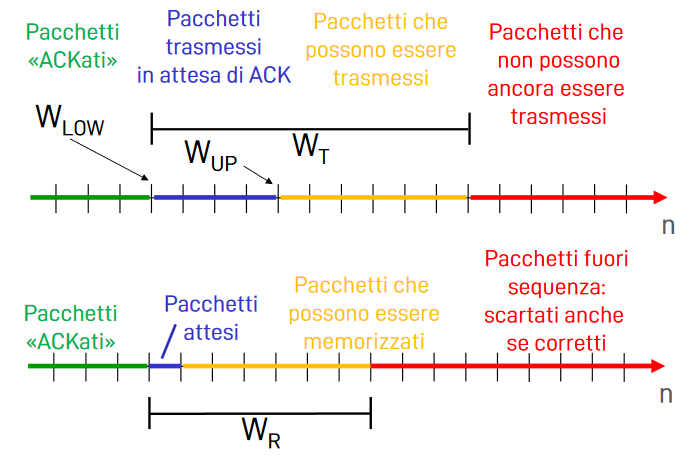
\includegraphics[width=0.5\textwidth]{03/finestrePipelining.png}
            \caption{Finestre di trasmissione e di ricezione}
        \end{figure}